\section{Casi d'uso}

\subsection{UC8 - Movimenti direzionali}
\begin{figure}[h!]\centering
    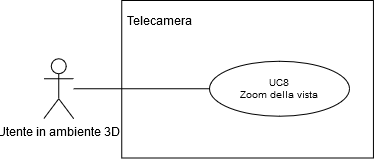
\includegraphics[scale=0.7]{template/images/UC8.png}
    \caption{UC8 - Movimenti direzionali}
\end{figure}
\begin{itemize}    
    \item \textbf{Attore:} utente;
    \item \textbf{Descrizione:} Compiere movimenti direzionali significa che, in ambiente di visualizzazione del grafico 3D, l'utente può interagire con il grafico compiendo degli spostamenti lungo i tre assi principali tramite comandi opportuni.
    \item \textbf{Precondizioni:}    
        \begin{itemize}
            \item Il caricamento del dataset è avvenuto con successo;
            \item La generazione dell'ambiente 3D e del relativo grafico non hanno riscontrato errori;
            \item Vengono eseguiti i comandi opportuni per i vari spostamenti.
        \end{itemize}    
    \item \textbf{Postcondizioni:}
        \begin{itemize}
            \item La telecamera che inquadra il grafico nell'ambiente 3D si troverà in una posizione diversa da quella in cui si trovava prima di compiere lo spostamento.
        \end{itemize}    
    \item \textbf{Scenario:} 
        \begin{itemize}
            \item L'utente interagisce con l'ambiente 3D per compiere un movimento direzionale.
        \end{itemize}
\end{itemize}
\subsubsection{UC8.1 - Movimento direzionale asse X}
\begin{itemize}    
    \item \textbf{Attore:} utente;
    \item \textbf{Descrizione:} L'utente interagisce opportunamente con l'ambiente 3D per spostarsi lungo l'asse X.
    \item \textbf{Precondizioni:}    
        \begin{itemize}
            \item Il caricamento del dataset è avvenuto con successo;
            \item La generazione dell'ambiente 3D e del relativo grafico non hanno riscontrato errori;
            \item Vengono eseguiti i comandi opportuni per lo spostamento lungo l'asse X.
        \end{itemize}    
    \item \textbf{Postcondizioni:}
        \begin{itemize}
            \item La telecamera che inquadra il grafico nell'ambiente 3D si troverà in una posizione diversa da quella in cui si trovava prima di compiere lo spostamento rispetto all'asse X.
        \end{itemize}    
    \item \textbf{Scenario:} 
        \begin{itemize}
            \item L'utente interagisce con l'ambiente 3D per compiere un movimento direzionale lungo l'asse X.
        \end{itemize}
\end{itemize}
\subsubsection{UC8.2 - Movimento direzionale asse Y}
\begin{itemize}    
    \item \textbf{Attore:} utente;
    \item \textbf{Descrizione:} L'utente interagisce opportunamente con l'ambiente 3D per spostarsi lungo l'asse Y.
    \item \textbf{Precondizioni:}   
        \begin{itemize}
            \item Il caricamento del dataset è avvenuto con successo;
            \item La generazione dell'ambiente 3D e del relativo grafico non hanno riscontrato errori;
            \item Vengono eseguiti i comandi opportuni per lo spostamento lungo l'asse Y.
        \end{itemize}    
    \item \textbf{Postcondizioni:}
        \begin{itemize}
            \item La telecamera che inquadra il grafico nell'ambiente 3D si troverà in una posizione diversa da quella in cui si trovava prima di compiere lo spostamento rispetto all'asse Y.
        \end{itemize}    
    \item \textbf{Scenario:} 
        \begin{itemize}
            \item L'utente interagisce con l'ambiente 3D per compiere un movimento direzionale lungo l'asse Y.
        \end{itemize}
\end{itemize}
\subsubsection{UC8.3 - Movimento direzionale asse Z}
\begin{itemize}    
    \item \textbf{Attore:} utente;
    \item \textbf{Descrizione:} L'utente interagisce opportunamente con l'ambiente 3D per spostarsi lungo l'asse Z.
    \item \textbf{Precondizioni:}    
        \begin{itemize}
            \item Il caricamento del dataset è avvenuto con successo;
            \item La generazione dell'ambiente 3D e del relativo grafico non hanno riscontrato errori;
            \item Vengono eseguiti i comandi opportuni per lo spostamento lungo l'asse Z.
        \end{itemize}    
    \item \textbf{Postcondizioni:}
        \begin{itemize}
            \item La telecamera che inquadra il grafico nell'ambiente 3D si troverà in una posizione diversa da quella in cui si trovava prima di compiere lo spostamento rispetto all'asse Z.
        \end{itemize}    
    \item \textbf{Scenario:} 
        \begin{itemize}
            \item L'utente interagisce con l'ambiente 3D per compiere un movimento direzionale lungo l'asse Z.
        \end{itemize}
\end{itemize}

\subsection{UC9 - Riposizionamento iniziale}
\begin{figure}[h!]\centering
    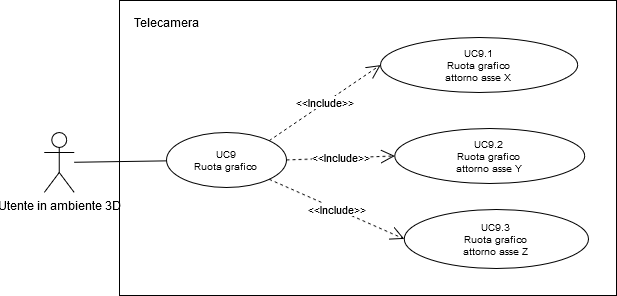
\includegraphics[scale=0.7]{template/images/UC9.png}
    \caption{UC9 - Riposizionamento iniziale}
\end{figure}
\begin{itemize}    
    \item \textbf{Attore:} utente;
    \item \textbf{Descrizione:} Riposizionare inizialmente la telecamera significa ripristinare la sua posizione e angolazione alla configurazione di partenza, annullando qualsiasi modifica apportata successivamente all'inizializzazione dell'ambiente 3D.
    \item \textbf{Precondizioni:}    
        \begin{itemize}
            \item Il caricamento del dataset è avvenuto con successo;
            \item La generazione dell'ambiente 3D e del relativo grafico non hanno riscontrato errori;
            \item Viene eseguito il comando opportuno per il riposizionamento iniziale.
        \end{itemize}    
    \item \textbf{Postcondizioni:}
        \begin{itemize}
            \item La posizione e angolazione della telecamera corrispondono alla configurazione di iniziale, uguale a quella di inizializzazione dell'ambiente 3D.
        \end{itemize}    
    \item \textbf{Scenario:} 
        \begin{itemize}
            \item L'utente interagisce con l'interfaccia per ripristinare la posizione e angolazione della telecamera ai valori iniziali.
        \end{itemize}
\end{itemize}

\subsection{UC10 - Visualizzare i valori di una barra del grafico}
\begin{figure}[h!]\centering
    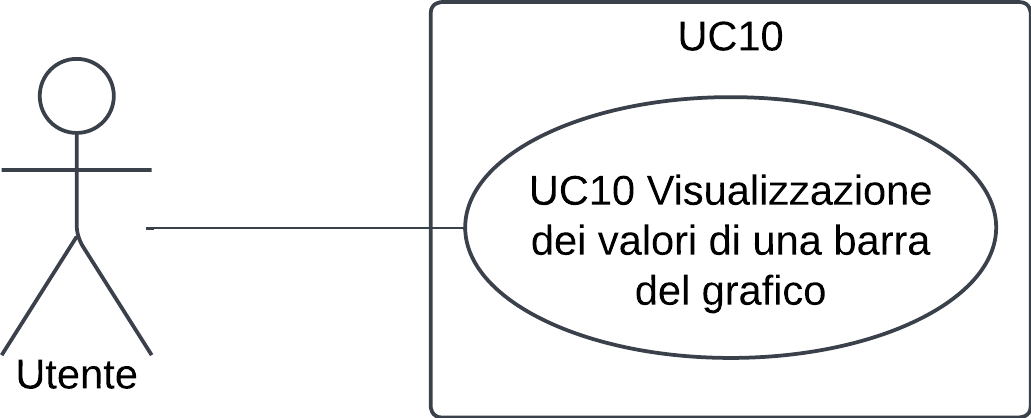
\includegraphics[scale=0.7]{template/images/UC10.png}
    \caption{UC10 - Visualizzare i valori di una barra del grafico}
\end{figure}
\begin{itemize}    
    \item \textbf{Attore:} utente;
    \item \textbf{Descrizione:} L'utente, tramite interazione opportuna, può selezionare una barra del grafico all'interno dell'ambiente 3D per visualizzarne i rispettivi valori.
    \item \textbf{Precondizioni:}    
        \begin{itemize}
            \item Il caricamento del dataset è avvenuto con successo;
            \item La generazione dell'ambiente 3D e del relativo grafico non hanno riscontrato errori;
            \item Viene eseguita l'interazione opportuna da parte dell'utente per la selezione della barra del grafico.
        \end{itemize}    
    \item \textbf{Postcondizioni:}
        \begin{itemize}
            \item Vengono visualizzati a schermo i valori della barra del grafico selezionata.
        \end{itemize}    
    \item \textbf{Scenario:} 
        \begin{itemize}
            \item L'utente interagisce con l'ambiente 3D e seleziona una barra del grafico per far apparire a schermo i valori.
        \end{itemize}
\end{itemize}

\subsection{UC11: Selezione elementi}
\begin{figure}[h!]\centering
    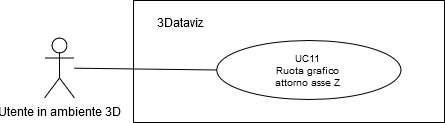
\includegraphics[scale=0.7]{template/images/UC11.png}
    \caption{UC11: Selezione elementi}
\end{figure}
\begin{itemize}    
    \item \textbf{Attore:} utente;
    \item \textbf{Descrizione:} L'utente, tramite interazione opportuna, può selezionare una barra del grafico all'interno dell'ambiente 3D oppure una singola cella nella tabella.
    \item \textbf{Precondizioni:}    
        \begin{itemize}
            \item Il caricamento del dataset è avvenuto con successo;
            \item La generazione dell'ambiente 3D e del relativo grafico non hanno riscontrato errori;
            \item La generazione della tabella non ha riscontrato errori;
            \item Viene eseguita l'interazione opportuna da parte dell'utente per la selezione.
        \end{itemize}    
    \item \textbf{Postcondizioni:}
        \begin{itemize}
            \item Viene evidenziata la selezione.
        \end{itemize}    
    \item \textbf{Scenario:} 
        \begin{itemize}
            \item L'utente interagisce con l'ambiente 3D e seleziona una barra del grafico oppure seleziona una cella della tabella.
        \end{itemize}
\end{itemize}

\pagebreak

\subsubsection{UC11.1: Selezione di un elemento del grafico}
\begin{figure}[h!]\centering
    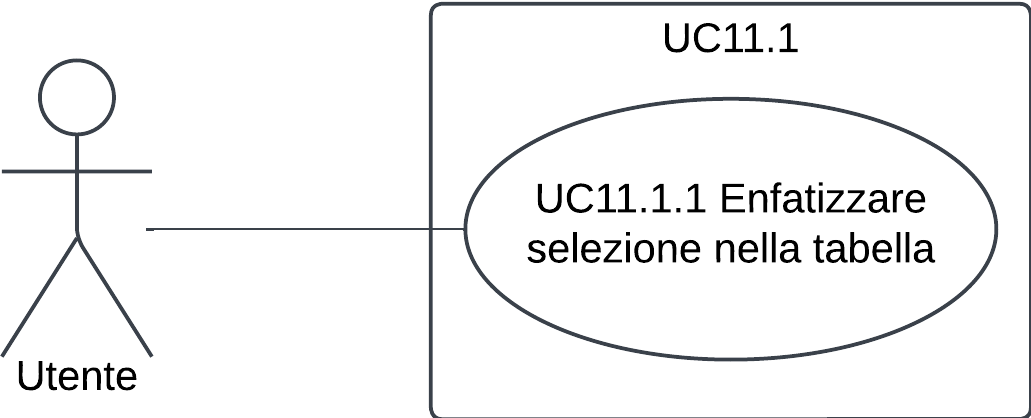
\includegraphics[scale=0.7]{template/images/UC11.1.png}
    \caption{UC11.1: Selezione di un elemento del grafico}
\end{figure}
\begin{itemize}    
    \item \textbf{Attore:} utente;
    \item \textbf{Descrizione:} L'utente può selezionare una barra del grafico 3D.
    \item \textbf{Precondizioni:}    
        \begin{itemize}
            \item Il caricamento del dataset è avvenuto con successo;
            \item La generazione dell'ambiente 3D e del relativo grafico non hanno riscontrato errori;
            \item Viene eseguita l'interazione opportuna da parte dell'utente per la selezione.
        \end{itemize}    
    \item \textbf{Postcondizioni:}
        \begin{itemize}
            \item Viene evidenziata della barra del grafico 3D.
        \end{itemize}    
    \item \textbf{Scenario:} 
        \begin{itemize}
            \item L'utente interagisce con il grafico 3D e seleziona una barra.
        \end{itemize}
\end{itemize}
\paragraph{UC11.1.1: Enfatizzare selezione nella tabella}
\begin{itemize}    
    \item \textbf{Attore:} utente;
    \item \textbf{Descrizione:} Viene evidenziata in maniera opportuna nella tabella la selezione compiuta dall'utente nel grafico 3D.
    \item \textbf{Precondizioni:}    
        \begin{itemize}
            \item Il caricamento del dataset è avvenuto con successo;
            \item La generazione della tabella non ha riscontrato errori;
            \item Viene eseguita l'interazione opportuna da parte dell'utente per la selezione.
        \end{itemize}    
    \item \textbf{Postcondizioni:}
        \begin{itemize}
            \item Viene evidenziata la cella nella tabella.
        \end{itemize}    
    \item \textbf{Scenario:} 
        \begin{itemize}
            \item L'utente interagisce con il grafico 3D, evidenziando la corrispondente cella della tabella.
        \end{itemize}
\end{itemize}

\pagebreak

\subsubsection{UC11.2: Selezione di una cella della tabella}
\begin{figure}[h!]\centering
    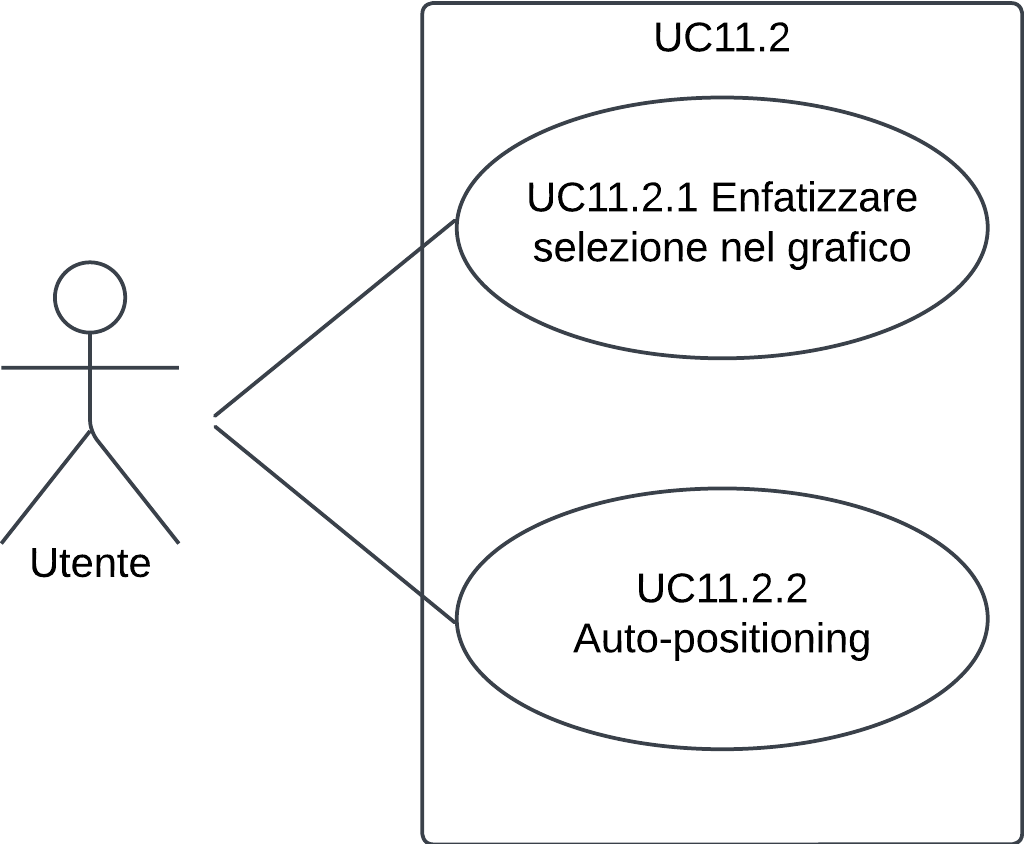
\includegraphics[scale=0.7]{template/images/UC11.2.png}
    \caption{UC11.2: Selezione di una cella della tabella}
\end{figure}
\begin{itemize}    
    \item \textbf{Attore:} utente;
    \item \textbf{Descrizione:} L'utente può selezionare una cella all'interno della tabella.
    \item \textbf{Precondizioni:}    
        \begin{itemize}
            \item Il caricamento del dataset è avvenuto con successo;
            \item La generazione della tabella non ha riscontrato errori;
            \item Viene eseguita l'interazione opportuna da parte dell'utente per la selezione della cella.
        \end{itemize}    
    \item \textbf{Postcondizioni:}
        \begin{itemize}
            \item Viene evidenziata la cella della tabella.
        \end{itemize}    
    \item \textbf{Scenario:} 
        \begin{itemize}
            \item L'utente interagisce con la tabella selezionando una cella la quale verrà evidenziata.
        \end{itemize}
\end{itemize}
\paragraph{UC11.2.1: Enfatizzare selezione nel grafico}
\begin{itemize}    
    \item \textbf{Attore:} utente;
    \item \textbf{Descrizione:} Viene evidenziata in maniera opportuna nel grafico 3D la selezione compiuta dall'utente nella tabella.
    \item \textbf{Precondizioni:}    
        \begin{itemize}
            \item Il caricamento del dataset è avvenuto con successo;
            \item La generazione dell'ambiente 3D e del relativo grafico non hanno riscontrato errori;
            \item Viene eseguita l'interazione opportuna da parte dell'utente per la selezione.
        \end{itemize}    
    \item \textbf{Postcondizioni:}
        \begin{itemize}
            \item Viene evidenziata la barra del grafico 3D.
        \end{itemize}    
    \item \textbf{Scenario:} 
        \begin{itemize}
            \item L'utente interagisce con una cella della tabella, evidenziando la corrispondente barra del grafico 3D.
        \end{itemize}
\end{itemize}
\paragraph{UC11.2.2: Auto-positioning}
\begin{itemize}    
    \item \textbf{Attore:} utente;
    \item \textbf{Descrizione:} In seguito alla selezione di una cella, la vista si sposta sulla corrispondente barra del grafico 3D, centrandola sullo schermo.
    \item \textbf{Precondizioni:}    
        \begin{itemize}
            \item Il caricamento del dataset è avvenuto con successo;
            \item La generazione dell'ambiente 3D e del relativo grafico non hanno riscontrato errori;
            \item Viene richiesta un'operazione di auto-positioning.
        \end{itemize}    
    \item \textbf{Postcondizioni:}
        \begin{itemize}
            \item La telecamera e la relativa inquadratura saranno in una posizione diversa da quella iniziale e avranno inoltre in primo piano la barra selezionata del grafico 3D.
        \end{itemize}    
    \item \textbf{Scenario:} 
        \begin{itemize}
            \item L'utente seleziona una cella della tabella e la telecamera nell'ambiente 3D si sposta di conseguenza inquadrando la corrispettiva barra del grafico.
        \end{itemize}
\end{itemize}

\subsection{UC12: Modifica trasparenza barra del grafico}
\begin{figure}[h!]\centering
    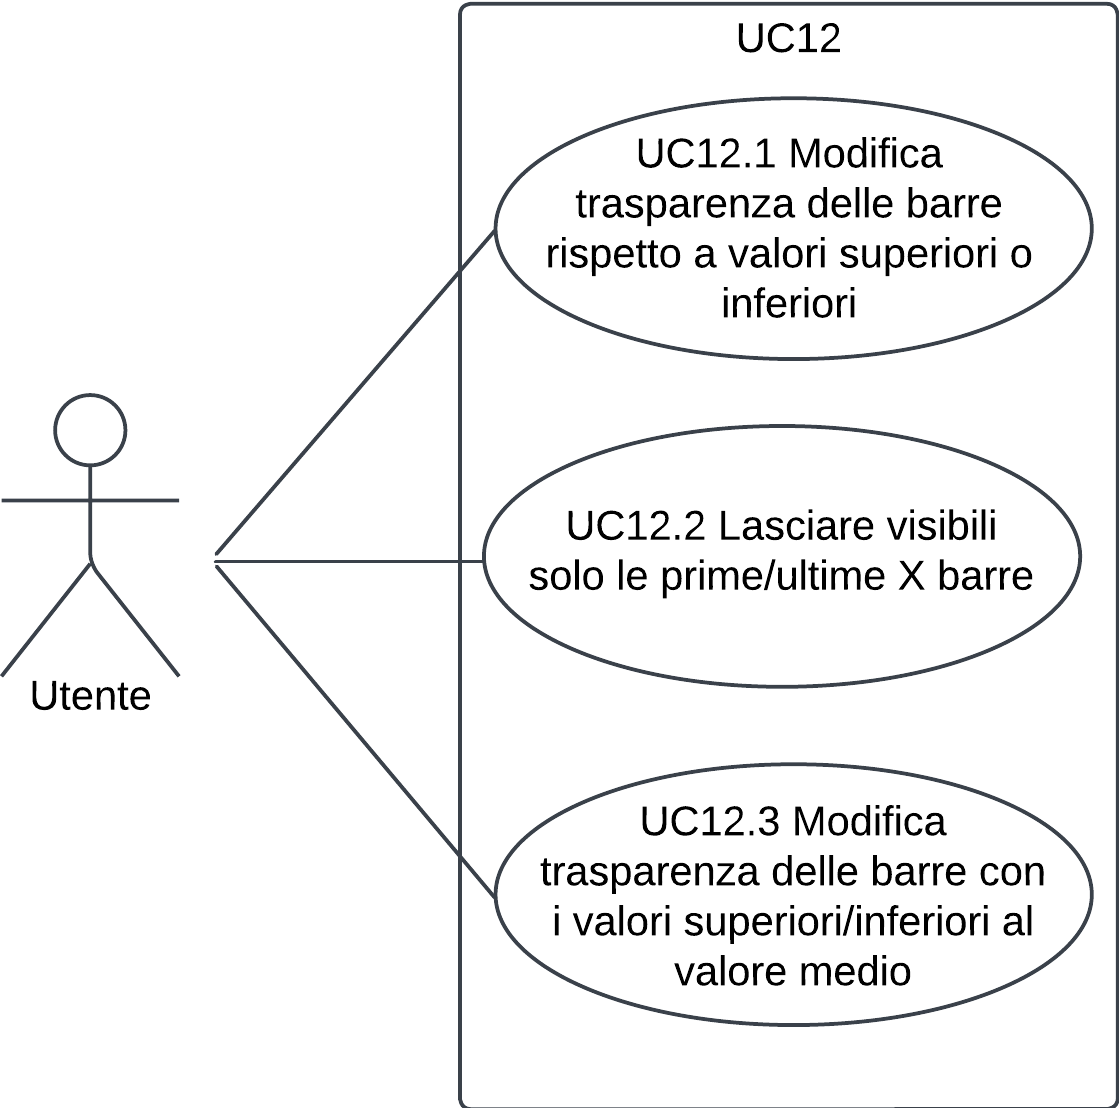
\includegraphics[scale=0.7]{template/images/UC12.png}
    \caption{Modifica trasparenza barra del grafico}
\end{figure}
\begin{itemize}    
    \item \textbf{Attore:} utente;
    \item \textbf{Descrizione:} Viene aumentata la trasparenza di una barra del grafico all'interno dell'ambiente 3D.
    \item \textbf{Precondizioni:}    
        \begin{itemize}
            \item Il caricamento del dataset è avvenuto con successo;
            \item La generazione dell'ambiente 3D e del relativo grafico non hanno riscontrato errori.
        \end{itemize}    
    \item \textbf{Postcondizioni:}
        \begin{itemize}
            \item Il valore di trasparenza delle altre barre del grafico 3D è maggiore rispetto a quello delle altre.
        \end{itemize}    
    \item \textbf{Scenario:} 
        \begin{itemize}
            \item L'utente evidenzia una determinata barra del grafico viene aumentato il valore di trasparenza a tutte le altre.
        \end{itemize}
\end{itemize}
\subsubsection{UC12.1: Opacizzare le barre rispetto a valori superiori o inferiori}
\begin{itemize}    
    \item \textbf{Attore:} utente;
    \item \textbf{Descrizione:} L'utente può stabilire un valore limite al di sopra o al di sotto del quale alcune barre verranno evidenziate.
    \item \textbf{Precondizioni:}    
        \begin{itemize}
            \item Il caricamento del dataset è avvenuto con successo;
            \item La generazione dell'ambiente 3D e del relativo grafico non hanno riscontrato errori;
            \item La generazione dell'interfaccia non ha riscontrato errori;
            \item L'utente imposta correttamente tutti i parametri necessari.
        \end{itemize}    
    \item \textbf{Postcondizioni:}
        \begin{itemize}
            \item Ogni barra selezionata nel grafico 3D viene resa più visibile rendendo le altre barre più trasparenti.
        \end{itemize}    
    \item \textbf{Scenario:} 
        \begin{itemize}
            \item L'utente interagisce con l'interfaccia selezionando il numero di barre con i valori più elevati o più bassi da evidenziare nel grafico 3D.
        \end{itemize}
\end{itemize}
\subsubsection{UC12.2: Lasciare visibili solo le prime/ultime X barre}
\begin{itemize}    
    \item \textbf{Attore:} utente;
    \item \textbf{Descrizione:} L'utente può evidenziare le X barre più piccole/grandi.
    \item \textbf{Precondizioni:}    
        \begin{itemize}
            \item Il caricamento del dataset è avvenuto con successo;
            \item La generazione dell'ambiente 3D e del relativo grafico non hanno riscontrato errori;
            \item La generazione dell'interfaccia non ha riscontrato errori;
            \item L'utente imposta correttamente tutti i parametri necessari.
        \end{itemize}    
    \item \textbf{Postcondizioni:}
        \begin{itemize}
            \item Ogni barra selezionata nel grafico 3D viene resa più visibile rendendo le altre barre più trasparenti.
        \end{itemize}    
    \item \textbf{Scenario:} 
        \begin{itemize}
            \item L'utente interagisce con l'interfaccia selezionando il numero di barre con i valori più elevati o più bassi da evidenziare nel grafico 3D.
        \end{itemize}
\end{itemize}
\subsubsection{UC12.3: Opacizzare le barre con i valori superiori/inferiori al valore medio}
\begin{itemize}    
    \item \textbf{Attore:} utente;
    \item \textbf{Descrizione:} L'utente può scegliere se evidenziare nel grafico 3D le barre il quale valore è superiore o inferiore al valore medio.
    \item \textbf{Precondizioni:}    
        \begin{itemize}
            \item Il caricamento del dataset è avvenuto con successo;
            \item La generazione dell'ambiente 3D e del relativo grafico non hanno riscontrato errori;
            \item La generazione dell'interfaccia non ha riscontrato errori;
            \item L'utente imposta correttamente tutti i parametri necessari.
        \end{itemize}    
    \item \textbf{Postcondizioni:}
        \begin{itemize}
            \item Ogni barra con il rispettivo valore superiore/inferiore al valore medio verrà opacizzata.
        \end{itemize}    
    \item \textbf{Scenario:} 
        \begin{itemize}
            \item L'utente interagisce con l'interfaccia per evidenziare nel grafico 3D solo le barre con un valore superiore o inferiore al valore medio.
        \end{itemize}
\end{itemize}

\subsection{UC13: Visualizzare un piano parallelo alla base}
\begin{figure}[h!]\centering
    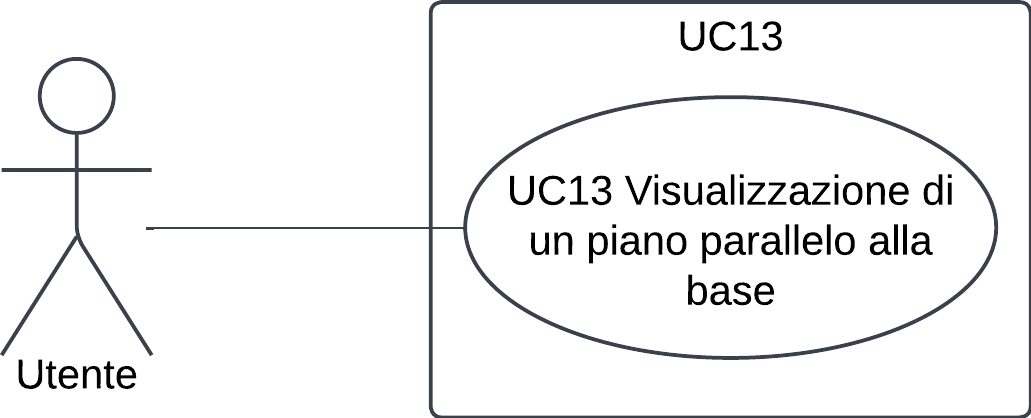
\includegraphics[scale=0.7]{template/images/UC13.png}
    \caption{UC13: Visualizzare un piano parallelo alla base}
\end{figure}
\begin{itemize}    
    \item \textbf{Attore:} utente;
    \item \textbf{Descrizione:} Un piano, parallelo alla base, viene inserito nel grafico 3D per evidenziare un valore di interesse, scelto dall'utente tra quelli ricavabili dai dati. Questo piano offre una rappresentazione visiva immediata del valore selezionato.
    \item \textbf{Precondizioni:}    
        \begin{itemize}
            \item Il caricamento del dataset è avvenuto con successo;
            \item La generazione dell'ambiente 3D e del relativo grafico non hanno riscontrato errori.
        \end{itemize}    
    \item \textbf{Postcondizioni:}
        \begin{itemize}
            \item Viene generato un piano, nel grafico 3D, parallelo alla base che evidenzia il valore di interesse scelto dall'utente.
        \end{itemize}    
    \item \textbf{Scenario:} 
        \begin{itemize}
            \item L'utente può evidenziare un determinato valore di interesse (ad esempio il valore medio) ed esso sarà rappresentato nel grafico dal piano generato.
        \end{itemize}
\end{itemize}

\pagebreak

\subsection{UC14: Visualizzazione errore nel caricamento del dataset}
\begin{figure}[h!]\centering
    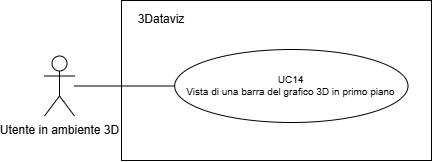
\includegraphics[scale=0.7]{template/images/UC14.png}
    \caption{UC14: Visualizzazione errore nel caricamento del dataset}
\end{figure}
\begin{itemize}    
    \item \textbf{Attore:} utente;
    \item \textbf{Descrizione:} L'utente visualizza un messaggio di errore dovuto al caricamento del dataset.
    \item \textbf{Precondizioni:}    
        \begin{itemize}
            \item L'utente ha selezionato il dataset da caricare;
            \item Il caricamento del dataset non è andato a buon fine.
        \end{itemize}    
    \item \textbf{Postcondizioni:}
        \begin{itemize}
            \item Viene visualizzato a schermo un messaggio di errore in seguito ad uno o più problemi riscontrati durante il caricamento del dataset selezionato.
        \end{itemize}    
    \item \textbf{Scenario:} 
        \begin{itemize}
            \item L'utente, in seguito al fallimento del caricamento del dataset selezionato, visualizza il messaggio di errore.
        \end{itemize}
\end{itemize}